
%	======= 1) NOW WHAT? =======

\begin{frame}
	\frametitle{Muy bien pero...¿Cómo sigo?}
	
	\begin{center}
		
\includegraphics[scale=0.40]{img/nowwhat.jpg}
	\end{center}

\end{frame}

%	======= 2) REQUISITOS =======

\begin{frame}
	\frametitle{¿Qué necesito?}
	
	Como has podido ver desarrollar un videojuego no es tarea fácil, requiere de un proceso de constante aprendizaje, investigación, dedicación y mucha ayuda.
		
	\begin{block}{Recomendaciones}
		\begin{itemize}
			\item \textbf{Motivación}: Hay que dedicarle mucho tiempo.
			\item \textbf{Curiosidad}: Interés por aprender cosas nuevas y mejorar lo que ya sabes.
			\item \textbf{Saber Inglés}: Gran cantidad de los recursos de calidad están en inglés.
			\item \textbf{Contactos}: Trabajo artístico, publicitario, sonido, beta testers...
			\item \textbf{Comunidad}: Lugar de referencia para consultar, compartir, etc.
		\end{itemize}
	\end{block}

\end{frame}

%	======= 3) LENGUAJES =======

\begin{frame}
	\frametitle{Lenguajes Alto Nivel}
	
	Según los conocimientos que tengas, así como los propósitos y metas del juego a desarrollar es importante elegir bien el lenguaje de programación.
		
	\begin{block}{Recomendaciones}
		\begin{itemize}
			\item C/C++/C\#
			\item Python
			\item Java
			\item Lua
			\item Ruby
		\end{itemize}
	\end{block}

\end{frame}

%	======= 4) LIBRERÍAS 2D =======

\begin{frame}
	\frametitle{Librerías 2D}
	La mejor forma de adentrarse en el desarrollo de videojuegos.
	\newline
	\begin{columns}[c]
		\column{100pt}
		\begin{block}{Algunos ejemplos destacados}
            \begin{itemize}
							\item Gosu
							\item SDL
							\item Allegro
							\item Pygame
							\item ClanLib
            \end{itemize}            
        \end{block}        
		\column{100pt}
		\begin{center}
			
\includegraphics[scale=0.32]{img/allegro.png}
			\newline
			\newline
			
\includegraphics[scale=0.22]{img/clanlib.png}
			\newline
			\newline
			
\includegraphics[scale=0.22]{img/pygame.png}
		\end{center}
		\column{100pt}
		\begin{center}
			
\includegraphics[scale=0.045]{img/sdl.png}
			\newline
			
\includegraphics[scale=0.23]{img/gosu.png}
		\end{center}
	\end{columns} 

\end{frame}

%	======= 5) LIBRERÍAS 3D =======

\begin{frame}
	\frametitle{Librerías 3D}
	El salto de calidad... 			\hspace{5.5cm}
\includegraphics[scale=0.12]{img/2dto3d.jpg}
	\newline
	\begin{columns}[c]
		\column{150pt}
		\begin{block}{Algunos ejemplos destacados}
            \begin{itemize}
							\item Ogre
							\item IrrLicht
							\item Crystal Space
							\item Panda
            \end{itemize}            
        \end{block}        
		\column{150pt}
		\begin{center}
			
\includegraphics[scale=0.30]{img/ogre.png}
			\hspace{0.20cm}
			
\includegraphics[scale=0.40]{img/crystal.png}
			\newline
			\newline
			
\includegraphics[scale=0.50]{img/panda.png}
			\hspace{0.60cm}
			
\includegraphics[scale=1.20]{img/irrlicht.png}
		\end{center}
	\end{columns} 

\end{frame}

%	======= 6) LIBRERÍAS AUXILIARES =======

\begin{frame}
	\frametitle{Otras Librerías y Herramientas}
		
	En muchas ocasiones es necesario apoyarse en otras librerías externas o herramientas que desarrollarán funciones auxiliares.
	\newline
	\begin{columns}[c]
		\column{150pt}
			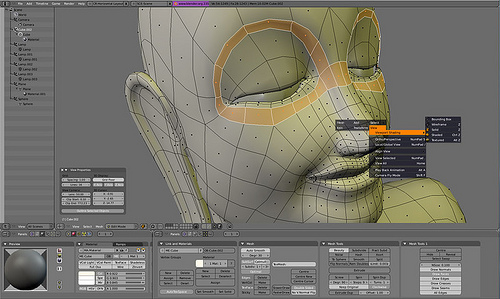
\includegraphics[scale=0.40]{img/blender.jpg}
		\column{150pt}
		\begin{block}{Algunos ejemplos destacados}
			\begin{itemize}
				\item Física: \emph{ODE, BULLET.}
				\item Gestión de Entrada: \emph{OIS.}
				\item Diseño Artístico: \emph{Gimp, Blender.}
				\newline
			\end{itemize}
		\end{block}
	\end{columns}

\end{frame}

%	======= 7) RECURSOS BIBLIOGRÁFICOS =======

\begin{frame}
	\frametitle{La biblioteca}
	
	\begin{center}
		
\includegraphics[scale=0.50]{img/biblio.jpg}
	\end{center}

\end{frame}

%	======= 8) TRABAJO EN EQUIPO =======

\begin{frame}
	\frametitle{Trabajo en Equipo}
	
	\begin{center}
		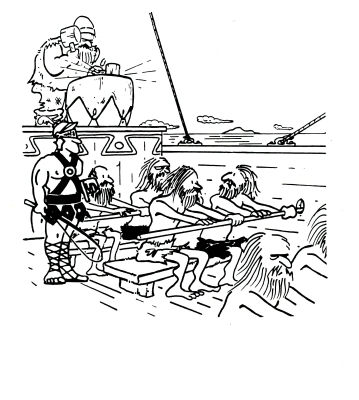
\includegraphics[scale=0.70]{img/equipo.jpg}
	\end{center}

\end{frame}

%	======= 9) VAYA TELA CON LA UCA: LABOON =======

\begin{frame}
	\frametitle{Algunos ejemplos del potencial existente}
	
	\begin{center}
		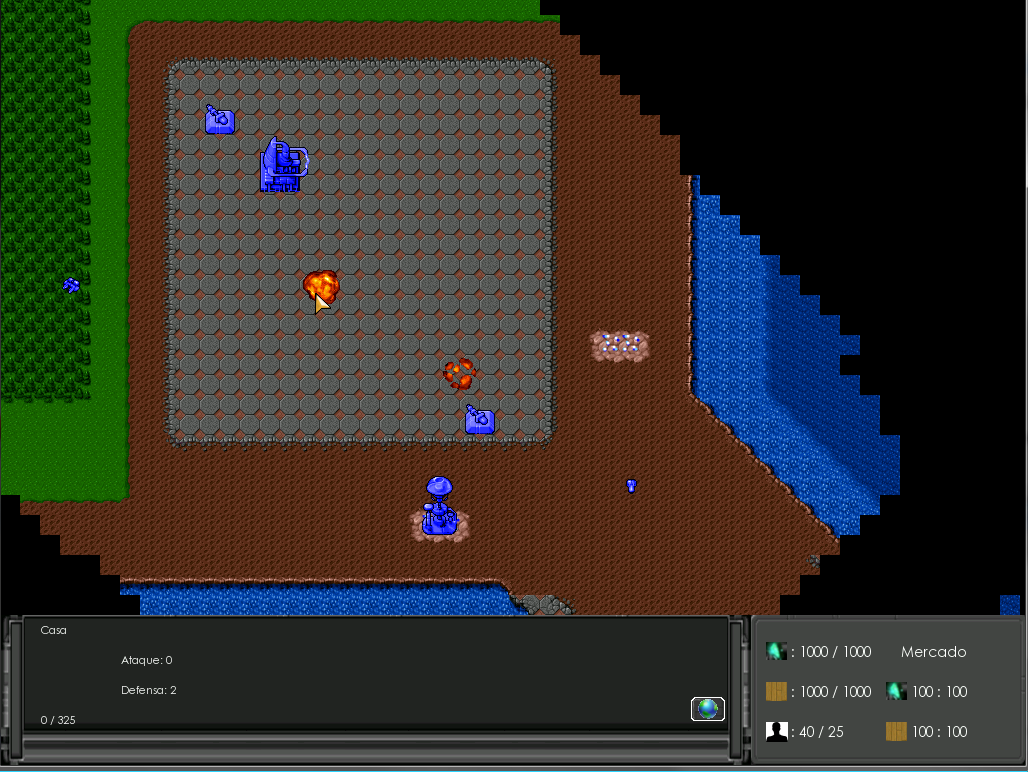
\includegraphics[scale=0.25]{img/laboon.png}
	\end{center}

\end{frame}

%	======= 10) VAYA TELA CON LA UCA: FREEPADEL =======

\begin{frame}
	\frametitle{Algunos ejemplos del potencial existente}
	
	\begin{center}
		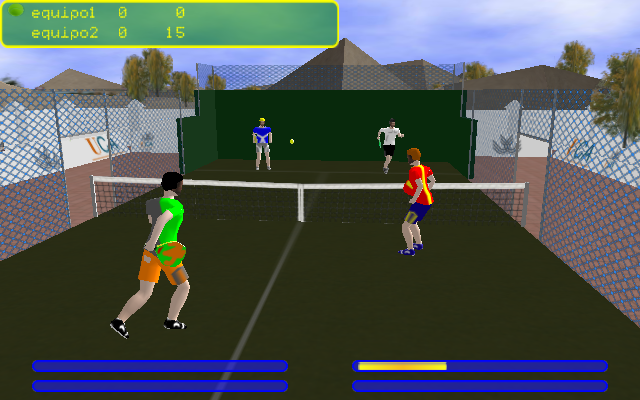
\includegraphics[scale=0.45]{img/freepadel.png}
	\end{center}

\end{frame}

%	======= 11) VAYA TELA CON LA UCA: AVIONES =======

\begin{frame}
	\frametitle{Algunos ejemplos del potencial existente}
	
	\begin{center}
		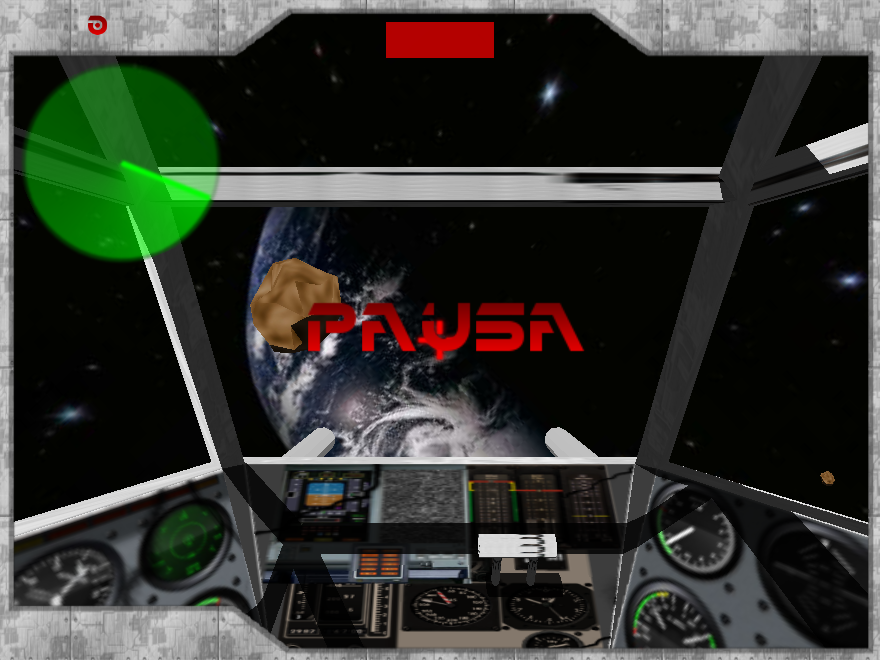
\includegraphics[scale=0.30]{img/avion.png}
	\end{center}

\end{frame}

%	======= 12) ADVUCA, TU AMIGO FIEL =======

\begin{frame}
	\frametitle{ADVUCA, tu amigo fiel}
		
	Desde la ADVUCA nos comprometemos a ofrecer ayuda para fomentar desarrollo de proyectos e incentivar el aprendizaje a través de los videojuegos.

	\begin{block}{Algunos ejemplos destacados}
		\begin{itemize}
			\item Formación de grupos de trabajo \emph{(juegos, manuales, etc).}
			\item Difusión.
			\item Consultas.
		\end{itemize}
	\end{block}

	\begin{center}
		
\includegraphics[scale=0.50]{img/micro.png}
	\end{center}

\end{frame}

%	======= 13) MUNDO LABORAL =======

\begin{frame}
	\frametitle{El Exteriooooor...}
		
	Después de la UCA, empieza lo bueno...
	\newline
	\begin{columns}[c]
		\column{150pt}
			\begin{block}{Algunas posibilidades}
				\begin{itemize}
					\item Masters.
					\item Desarrolladoras de Videojuegos.
					\item Centros Multimedia.
				\end{itemize}
			\end{block}
		\column{150pt}
			\begin{center}
				
\includegraphics[scale=0.15]{img/exterior.jpg}
			\end{center}
	\end{columns}
\end{frame}

%	======= 14) DEJATE DE ROYOS Y NO TE QUEDES MÁS CONMIGO =======

\begin{frame}
	\frametitle{Pero... ¿de verdad?}
	\begin{center}
		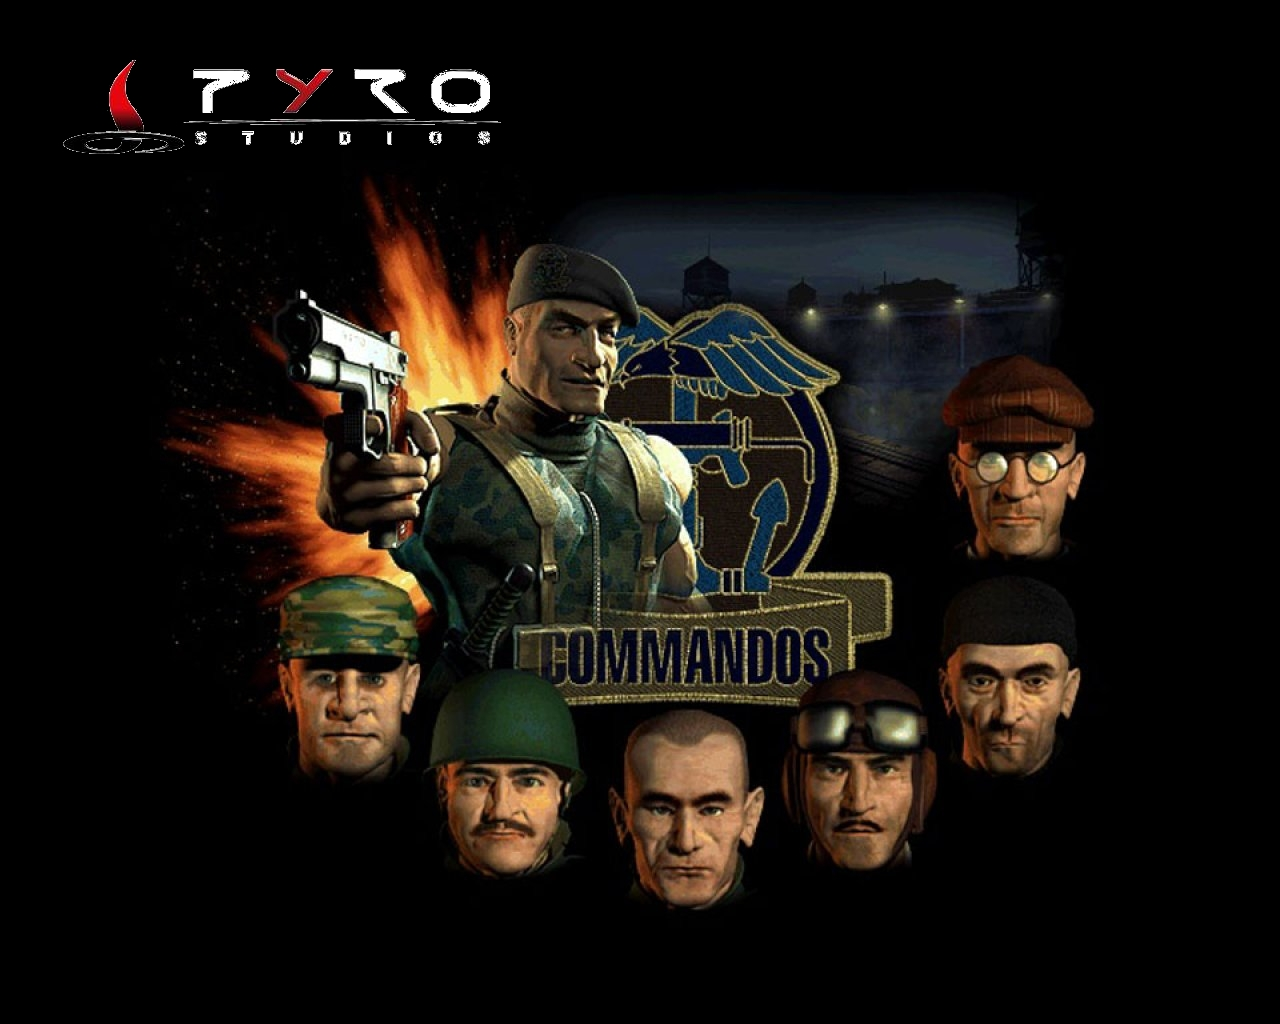
\includegraphics[scale=0.20]{img/comandos.jpeg}
	\end{center}
\end{frame}




